\documentclass{standalone}
\usepackage{tikz}
\usetikzlibrary{patterns, positioning}


\begin{document}
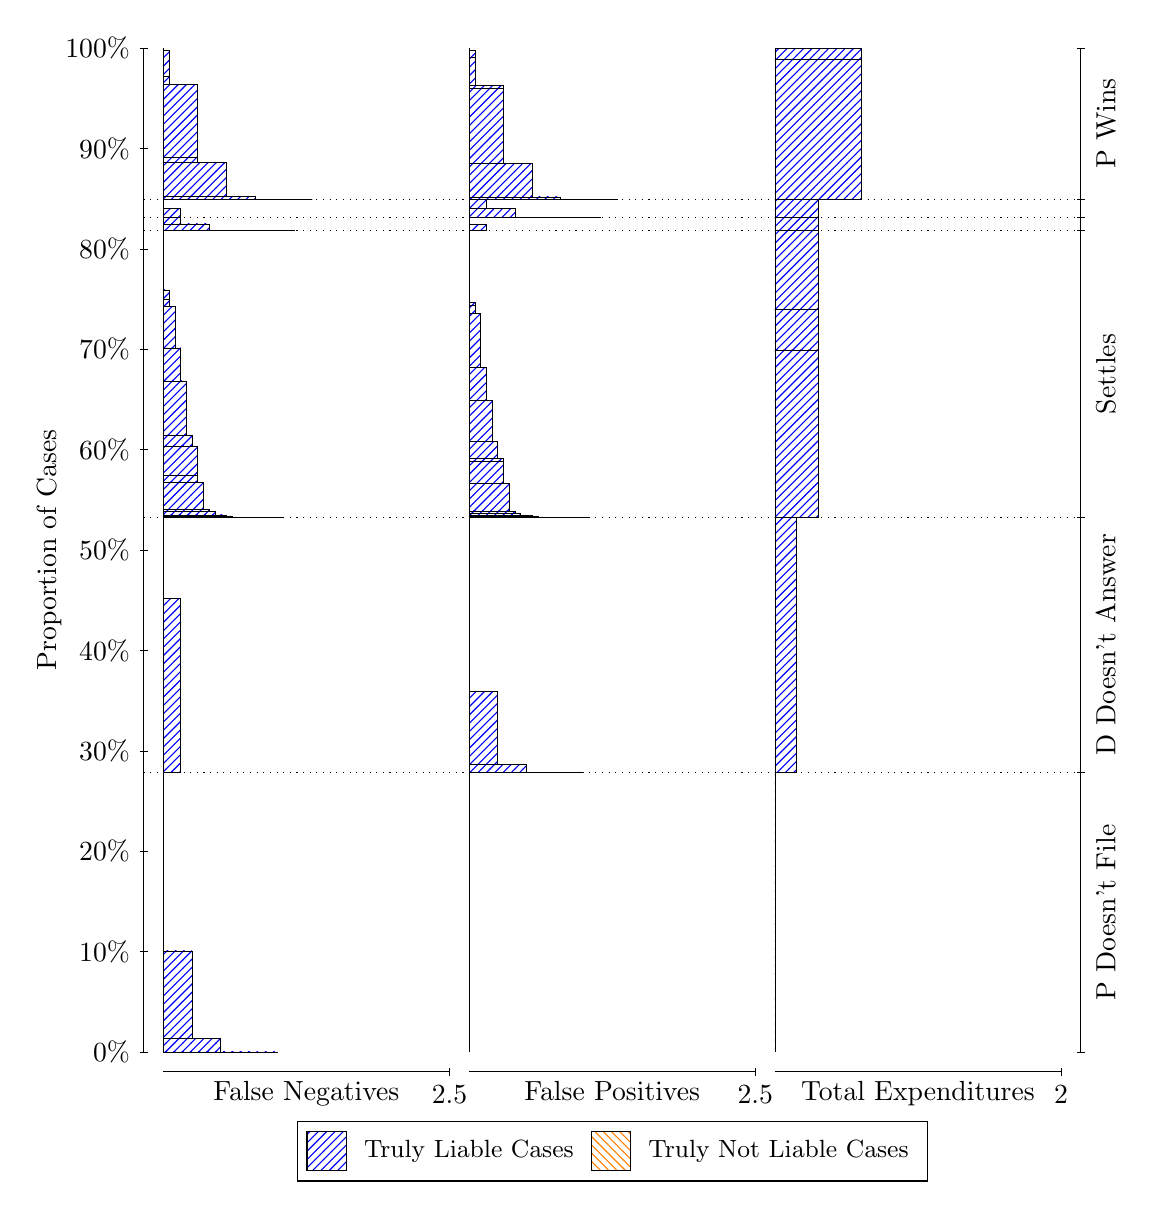
\begin{tikzpicture}
\draw[black, very thin] (1.5,1.75) -- (1.5,14.5);
\node[rotate=90, text=black, anchor=center] at (0.3, 8.125) {Proportion of Cases};
\draw[black, very thin] (1.45,1.75) -- (1.55,1.75);
\node[text=black, anchor=east] at (1.45, 1.75) {0\%};
\draw[black, very thin] (1.45,3.025) -- (1.55,3.025);
\node[text=black, anchor=east] at (1.45, 3.025) {10\%};
\draw[black, very thin] (1.45,4.3) -- (1.55,4.3);
\node[text=black, anchor=east] at (1.45, 4.3) {20\%};
\draw[black, very thin] (1.45,5.575) -- (1.55,5.575);
\node[text=black, anchor=east] at (1.45, 5.575) {30\%};
\draw[black, very thin] (1.45,6.85) -- (1.55,6.85);
\node[text=black, anchor=east] at (1.45, 6.85) {40\%};
\draw[black, very thin] (1.45,8.125) -- (1.55,8.125);
\node[text=black, anchor=east] at (1.45, 8.125) {50\%};
\draw[black, very thin] (1.45,9.4) -- (1.55,9.4);
\node[text=black, anchor=east] at (1.45, 9.4) {60\%};
\draw[black, very thin] (1.45,10.675) -- (1.55,10.675);
\node[text=black, anchor=east] at (1.45, 10.675) {70\%};
\draw[black, very thin] (1.45,11.95) -- (1.55,11.95);
\node[text=black, anchor=east] at (1.45, 11.95) {80\%};
\draw[black, very thin] (1.45,13.225) -- (1.55,13.225);
\node[text=black, anchor=east] at (1.45, 13.225) {90\%};
\draw[black, very thin] (1.45,14.5) -- (1.55,14.5);
\node[text=black, anchor=east] at (1.45, 14.5) {100\%};

\draw[black, very thin] (13.4,1.75) -- (13.4,14.5);
\draw[black, very thin] (13.35,1.75) -- (13.45,1.75);
\node[anchor=west] at (13.35, 1.75) {};
\draw[black, very thin] (13.35,5.2972) -- (13.45,5.2972);
\node[anchor=west] at (13.35, 5.2972) {};
\draw[black, very thin] (13.35,8.5405) -- (13.45,8.5405);
\node[anchor=west] at (13.35, 8.5405) {};
\draw[black, very thin] (13.35,12.182) -- (13.45,12.182);
\node[anchor=west] at (13.35, 12.182) {};
\draw[black, very thin] (13.35,12.349) -- (13.45,12.349);
\node[anchor=west] at (13.35, 12.349) {};
\draw[black, very thin] (13.35,12.577) -- (13.45,12.577);
\node[anchor=west] at (13.35, 12.577) {};
\draw[black, very thin] (13.35,14.5) -- (13.45,14.5);
\node[anchor=west] at (13.35, 14.5) {};

\draw[black, very thin, pattern color=blue, pattern=north east lines] (1.75,1.75) rectangle (3.2033,1.75);
\draw[black, very thin, pattern color=blue, pattern=north east lines] (1.75,1.75) rectangle (2.84,1.7514);
\draw[black, very thin, pattern color=blue, pattern=north east lines] (1.75,1.7514) rectangle (2.4767,1.9189);
\draw[black, very thin, pattern color=blue, pattern=north east lines] (1.75,1.9189) rectangle (2.1133,3.0332);
\draw[black, very thin, pattern color=orange, pattern=north west lines] (1.75,3.0332) rectangle (1.75,3.0332);
\draw[black, very thin, pattern color=blue, pattern=north east lines] (1.75,3.0332) rectangle (1.75,5.2972);
\draw[black, very thin, pattern color=blue, pattern=north east lines] (1.75,5.2972) rectangle (1.968,7.5091);
\draw[black, very thin, pattern color=orange, pattern=north west lines] (1.75,7.5091) rectangle (1.75,7.5091);
\draw[black, very thin, pattern color=blue, pattern=north east lines] (1.75,7.5091) rectangle (1.75,8.5405);
\draw[black, very thin, pattern color=blue, pattern=north east lines] (1.75,8.5405) rectangle (3.276,8.5405);
\draw[black, very thin, pattern color=blue, pattern=north east lines] (1.75,8.5405) rectangle (2.9853,8.5405);
\draw[black, very thin, pattern color=blue, pattern=north east lines] (1.75,8.5405) rectangle (2.9127,8.5405);
\draw[black, very thin, pattern color=blue, pattern=north east lines] (1.75,8.5405) rectangle (2.84,8.5405);
\draw[black, very thin, pattern color=blue, pattern=north east lines] (1.75,8.5405) rectangle (2.6947,8.5405);
\draw[black, very thin, pattern color=blue, pattern=north east lines] (1.75,8.5405) rectangle (2.622,8.5502);
\draw[black, very thin, pattern color=blue, pattern=north east lines] (1.75,8.5502) rectangle (2.5493,8.5711);
\draw[black, very thin, pattern color=blue, pattern=north east lines] (1.75,8.5711) rectangle (2.4767,8.5716);
\draw[black, very thin, pattern color=blue, pattern=north east lines] (1.75,8.5716) rectangle (2.404,8.6119);
\draw[black, very thin, pattern color=blue, pattern=north east lines] (1.75,8.6119) rectangle (2.3313,8.6387);
\draw[black, very thin, pattern color=blue, pattern=north east lines] (1.75,8.6387) rectangle (2.2587,8.9906);
\draw[black, very thin, pattern color=blue, pattern=north east lines] (1.75,8.9906) rectangle (2.186,9.0716);
\draw[black, very thin, pattern color=blue, pattern=north east lines] (1.75,9.0716) rectangle (2.186,9.4461);
\draw[black, very thin, pattern color=blue, pattern=north east lines] (1.75,9.4461) rectangle (2.1133,9.5882);
\draw[black, very thin, pattern color=blue, pattern=north east lines] (1.75,9.5882) rectangle (2.0407,10.273);
\draw[black, very thin, pattern color=blue, pattern=north east lines] (1.75,10.273) rectangle (1.968,10.692);
\draw[black, very thin, pattern color=blue, pattern=north east lines] (1.75,10.692) rectangle (1.8953,11.218);
\draw[black, very thin, pattern color=blue, pattern=north east lines] (1.75,11.218) rectangle (1.8227,11.307);
\draw[black, very thin, pattern color=blue, pattern=north east lines] (1.75,11.307) rectangle (1.8227,11.429);
\draw[black, very thin, pattern color=blue, pattern=north east lines] (1.75,11.429) rectangle (1.75,11.464);
\draw[black, very thin, pattern color=orange, pattern=north west lines] (1.75,11.464) rectangle (1.75,11.464);
\draw[black, very thin, pattern color=blue, pattern=north east lines] (1.75,11.464) rectangle (1.75,12.182);
\draw[black, very thin, pattern color=blue, pattern=north east lines] (1.75,12.182) rectangle (3.4213,12.182);
\draw[black, very thin, pattern color=blue, pattern=north east lines] (1.75,12.182) rectangle (3.058,12.182);
\draw[black, very thin, pattern color=blue, pattern=north east lines] (1.75,12.182) rectangle (2.6947,12.183);
\draw[black, very thin, pattern color=blue, pattern=north east lines] (1.75,12.183) rectangle (2.3313,12.268);
\draw[black, very thin, pattern color=blue, pattern=north east lines] (1.75,12.268) rectangle (1.968,12.349);
\draw[black, very thin, pattern color=orange, pattern=north west lines] (1.75,12.349) rectangle (1.75,12.349);
\draw[black, very thin, pattern color=blue, pattern=north east lines] (1.75,12.349) rectangle (1.968,12.459);
\draw[black, very thin, pattern color=orange, pattern=north west lines] (1.75,12.459) rectangle (1.75,12.459);
\draw[black, very thin, pattern color=blue, pattern=north east lines] (1.75,12.459) rectangle (1.75,12.577);
\draw[black, very thin, pattern color=blue, pattern=north east lines] (1.75,12.577) rectangle (3.6393,12.577);
\draw[black, very thin, pattern color=blue, pattern=north east lines] (1.75,12.577) rectangle (3.276,12.577);
\draw[black, very thin, pattern color=blue, pattern=north east lines] (1.75,12.577) rectangle (2.9127,12.612);
\draw[black, very thin, pattern color=blue, pattern=north east lines] (1.75,12.612) rectangle (2.5493,13.052);
\draw[black, very thin, pattern color=blue, pattern=north east lines] (1.75,13.052) rectangle (2.186,13.113);
\draw[black, very thin, pattern color=blue, pattern=north east lines] (1.75,13.113) rectangle (2.186,14.038);
\draw[black, very thin, pattern color=blue, pattern=north east lines] (1.75,14.038) rectangle (1.8227,14.136);
\draw[black, very thin, pattern color=blue, pattern=north east lines] (1.75,14.136) rectangle (1.8227,14.468);
\draw[black, very thin, pattern color=orange, pattern=north west lines] (1.75,14.468) rectangle (1.75,14.468);
\draw[black, very thin, pattern color=blue, pattern=north east lines] (1.75,14.468) rectangle (1.75,14.5);
\draw[black, very thin, pattern color=orange, pattern=north west lines] (5.6333,1.75) rectangle (5.6333,1.75);
\draw[black, very thin, pattern color=blue, pattern=north east lines] (5.6333,1.75) rectangle (5.6333,5.2972);
\draw[black, very thin, pattern color=orange, pattern=north west lines] (5.6333,5.2972) rectangle (7.0867,5.2972);
\draw[black, very thin, pattern color=blue, pattern=north east lines] (5.6333,5.2972) rectangle (7.0867,5.2972);
\draw[black, very thin, pattern color=blue, pattern=north east lines] (5.6333,5.2972) rectangle (6.7233,5.2975);
\draw[black, very thin, pattern color=blue, pattern=north east lines] (5.6333,5.2975) rectangle (6.36,5.4057);
\draw[black, very thin, pattern color=blue, pattern=north east lines] (5.6333,5.4057) rectangle (5.9967,6.3286);
\draw[black, very thin, pattern color=blue, pattern=north east lines] (5.6333,6.3286) rectangle (5.6333,8.5405);
\draw[black, very thin, pattern color=orange, pattern=north west lines] (5.6333,8.5405) rectangle (7.1593,8.5405);
\draw[black, very thin, pattern color=blue, pattern=north east lines] (5.6333,8.5405) rectangle (7.1593,8.5405);
\draw[black, very thin, pattern color=orange, pattern=north west lines] (5.6333,8.5405) rectangle (6.8687,8.5405);
\draw[black, very thin, pattern color=blue, pattern=north east lines] (5.6333,8.5405) rectangle (6.8687,8.5405);
\draw[black, very thin, pattern color=blue, pattern=north east lines] (5.6333,8.5405) rectangle (6.796,8.5405);
\draw[black, very thin, pattern color=orange, pattern=north west lines] (5.6333,8.5405) rectangle (6.7233,8.5405);
\draw[black, very thin, pattern color=blue, pattern=north east lines] (5.6333,8.5405) rectangle (6.7233,8.5405);
\draw[black, very thin, pattern color=orange, pattern=north west lines] (5.6333,8.5405) rectangle (6.578,8.5405);
\draw[black, very thin, pattern color=blue, pattern=north east lines] (5.6333,8.5405) rectangle (6.578,8.5405);
\draw[black, very thin, pattern color=blue, pattern=north east lines] (5.6333,8.5405) rectangle (6.5053,8.5501);
\draw[black, very thin, pattern color=blue, pattern=north east lines] (5.6333,8.5501) rectangle (6.4327,8.567);
\draw[black, very thin, pattern color=orange, pattern=north west lines] (5.6333,8.567) rectangle (6.4327,8.567);
\draw[black, very thin, pattern color=blue, pattern=north east lines] (5.6333,8.567) rectangle (6.4327,8.5671);
\draw[black, very thin, pattern color=blue, pattern=north east lines] (5.6333,8.5671) rectangle (6.36,8.5676);
\draw[black, very thin, pattern color=orange, pattern=north west lines] (5.6333,8.5676) rectangle (6.2873,8.5676);
\draw[black, very thin, pattern color=blue, pattern=north east lines] (5.6333,8.5676) rectangle (6.2873,8.5949);
\draw[black, very thin, pattern color=blue, pattern=north east lines] (5.6333,8.5949) rectangle (6.2147,8.6221);
\draw[black, very thin, pattern color=blue, pattern=north east lines] (5.6333,8.6221) rectangle (6.142,8.9668);
\draw[black, very thin, pattern color=blue, pattern=north east lines] (5.6333,8.9668) rectangle (6.0693,9.2576);
\draw[black, very thin, pattern color=blue, pattern=north east lines] (5.6333,9.2576) rectangle (6.0693,9.2928);
\draw[black, very thin, pattern color=orange, pattern=north west lines] (5.6333,9.2928) rectangle (5.9967,9.2928);
\draw[black, very thin, pattern color=blue, pattern=north east lines] (5.6333,9.2928) rectangle (5.9967,9.5044);
\draw[black, very thin, pattern color=blue, pattern=north east lines] (5.6333,9.5044) rectangle (5.924,10.03);
\draw[black, very thin, pattern color=blue, pattern=north east lines] (5.6333,10.03) rectangle (5.8513,10.449);
\draw[black, very thin, pattern color=blue, pattern=north east lines] (5.6333,10.449) rectangle (5.7787,11.134);
\draw[black, very thin, pattern color=blue, pattern=north east lines] (5.6333,11.134) rectangle (5.706,11.229);
\draw[black, very thin, pattern color=blue, pattern=north east lines] (5.6333,11.229) rectangle (5.706,11.276);
\draw[black, very thin, pattern color=blue, pattern=north east lines] (5.6333,11.276) rectangle (5.6333,12.182);
\draw[black, very thin, pattern color=orange, pattern=north west lines] (5.6333,12.182) rectangle (5.8513,12.182);
\draw[black, very thin, pattern color=blue, pattern=north east lines] (5.6333,12.182) rectangle (5.8513,12.263);
\draw[black, very thin, pattern color=blue, pattern=north east lines] (5.6333,12.263) rectangle (5.6333,12.349);
\draw[black, very thin, pattern color=orange, pattern=north west lines] (5.6333,12.349) rectangle (7.3047,12.349);
\draw[black, very thin, pattern color=blue, pattern=north east lines] (5.6333,12.349) rectangle (7.3047,12.349);
\draw[black, very thin, pattern color=blue, pattern=north east lines] (5.6333,12.349) rectangle (6.9413,12.349);
\draw[black, very thin, pattern color=blue, pattern=north east lines] (5.6333,12.349) rectangle (6.578,12.351);
\draw[black, very thin, pattern color=blue, pattern=north east lines] (5.6333,12.351) rectangle (6.2147,12.467);
\draw[black, very thin, pattern color=blue, pattern=north east lines] (5.6333,12.467) rectangle (5.8513,12.577);
\draw[black, very thin, pattern color=orange, pattern=north west lines] (5.6333,12.577) rectangle (7.5227,12.577);
\draw[black, very thin, pattern color=blue, pattern=north east lines] (5.6333,12.577) rectangle (7.5227,12.577);
\draw[black, very thin, pattern color=orange, pattern=north west lines] (5.6333,12.577) rectangle (7.1593,12.577);
\draw[black, very thin, pattern color=blue, pattern=north east lines] (5.6333,12.577) rectangle (7.1593,12.577);
\draw[black, very thin, pattern color=orange, pattern=north west lines] (5.6333,12.577) rectangle (6.796,12.577);
\draw[black, very thin, pattern color=blue, pattern=north east lines] (5.6333,12.577) rectangle (6.796,12.609);
\draw[black, very thin, pattern color=orange, pattern=north west lines] (5.6333,12.609) rectangle (6.4327,12.609);
\draw[black, very thin, pattern color=blue, pattern=north east lines] (5.6333,12.609) rectangle (6.4327,13.039);
\draw[black, very thin, pattern color=blue, pattern=north east lines] (5.6333,13.039) rectangle (6.0693,13.988);
\draw[black, very thin, pattern color=orange, pattern=north west lines] (5.6333,13.988) rectangle (6.0693,13.988);
\draw[black, very thin, pattern color=blue, pattern=north east lines] (5.6333,13.988) rectangle (6.0693,14.025);
\draw[black, very thin, pattern color=blue, pattern=north east lines] (5.6333,14.025) rectangle (5.706,14.377);
\draw[black, very thin, pattern color=blue, pattern=north east lines] (5.6333,14.377) rectangle (5.706,14.466);
\draw[black, very thin, pattern color=blue, pattern=north east lines] (5.6333,14.466) rectangle (5.6333,14.5);
\draw[black, very thin, pattern color=orange, pattern=north west lines] (9.5167,1.75) rectangle (9.5167,1.75);
\draw[black, very thin, pattern color=blue, pattern=north east lines] (9.5167,1.75) rectangle (9.5167,5.2972);
\draw[black, very thin, pattern color=orange, pattern=north west lines] (9.5167,5.2972) rectangle (9.7892,5.2972);
\draw[black, very thin, pattern color=blue, pattern=north east lines] (9.5167,5.2972) rectangle (9.7892,8.5405);
\draw[black, very thin, pattern color=orange, pattern=north west lines] (9.5167,8.5405) rectangle (10.062,8.5405);
\draw[black, very thin, pattern color=blue, pattern=north east lines] (9.5167,8.5405) rectangle (10.062,10.666);
\draw[black, very thin, pattern color=orange, pattern=north west lines] (9.5167,10.666) rectangle (10.062,10.666);
\draw[black, very thin, pattern color=blue, pattern=north east lines] (9.5167,10.666) rectangle (10.062,11.184);
\draw[black, very thin, pattern color=orange, pattern=north west lines] (9.5167,11.184) rectangle (10.062,11.184);
\draw[black, very thin, pattern color=blue, pattern=north east lines] (9.5167,11.184) rectangle (10.062,12.182);
\draw[black, very thin, pattern color=orange, pattern=north west lines] (9.5167,12.182) rectangle (10.062,12.182);
\draw[black, very thin, pattern color=blue, pattern=north east lines] (9.5167,12.182) rectangle (10.062,12.349);
\draw[black, very thin, pattern color=orange, pattern=north west lines] (9.5167,12.349) rectangle (10.062,12.349);
\draw[black, very thin, pattern color=blue, pattern=north east lines] (9.5167,12.349) rectangle (10.062,12.577);
\draw[black, very thin, pattern color=orange, pattern=north west lines] (9.5167,12.577) rectangle (10.607,12.577);
\draw[black, very thin, pattern color=blue, pattern=north east lines] (9.5167,12.577) rectangle (10.607,14.352);
\draw[black, very thin, pattern color=orange, pattern=north west lines] (9.5167,14.352) rectangle (10.607,14.352);
\draw[black, very thin, pattern color=blue, pattern=north east lines] (9.5167,14.352) rectangle (10.607,14.5);
\draw[black, dotted] (1.5,5.2972) -- (13.4,5.2972);
\draw[black, dotted] (1.5,8.5405) -- (13.4,8.5405);
\draw[black, dotted] (1.5,12.182) -- (13.4,12.182);
\draw[black, dotted] (1.5,12.349) -- (13.4,12.349);
\draw[black, dotted] (1.5,12.577) -- (13.4,12.577);
\draw[black, very thin] (1.75,1.5) -- (5.3833,1.5);
\node[text=black, anchor=north] at (3.5667, 1.5) {False Negatives};
\draw[black, very thin] (5.3833,1.45) -- (5.3833,1.55);
\node[text=black, anchor=north] at (5.3833, 1.45) {2.5};

\draw[black, very thin] (5.6333,1.5) -- (9.2667,1.5);
\node[text=black, anchor=north] at (7.45, 1.5) {False Positives};
\draw[black, very thin] (9.2667,1.45) -- (9.2667,1.55);
\node[text=black, anchor=north] at (9.2667, 1.45) {2.5};

\draw[black, very thin] (9.5167,1.5) -- (13.15,1.5);
\node[text=black, anchor=north] at (11.333, 1.5) {Total Expenditures};
\draw[black, very thin] (13.15,1.45) -- (13.15,1.55);
\node[text=black, anchor=north] at (13.15, 1.45) {2};

\node[text=black, centered, rotate=90] at (13.72, 3.5236) {P Doesn't File};
\node[text=black, centered, rotate=90] at (13.72, 6.9189) {D Doesn't Answer};
\node[text=black, centered, rotate=90] at (13.72, 10.361) {Settles};


\node[text=black, centered, rotate=90] at (13.72, 13.539) {P Wins};

\draw (7.449999999999999,1.5) node[draw=none] (baseCoordinate) {};
\begin{scope}[align=center]
        \matrix[scale=0.5, draw=black, below=0.5cm of baseCoordinate, nodes={draw}, column sep=0.1cm]{
            \node[rectangle, draw, minimum width=0.5cm, minimum height=0.5cm, pattern color=blue, pattern=north east lines] {}; &
            \node[draw=none, font=\small, text=black] (B) {Truly Liable Cases}; &
            \node[rectangle, draw, minimum width=0.5cm, minimum height=0.5cm, pattern color=orange, pattern=north west lines] {}; &
            \node[draw=none, font=\small, text=black] (B) {Truly Not Liable Cases}; \\
            };
\end{scope}

\end{tikzpicture}
\end{document}